%\PassOptionsToPackage{table}{xcolor}
% \documentclass[smaller, dvipsnames,%handout,
% hyperref={colorlinks=true,urlcolor=magenta,citecolor=cyan,linkcolor=orange}]{beamer}
\def\bmode{2} % Mode 0 for presentation, mode 1 for a handout with notes, mode 2 fo% r handout without notes
\if 0\bmode
\documentclass[usenames,dvipsnames,smaller]{beamer}
\else \if 1\bmode
\immediate\write18{pdflatex -jobname=\jobname-Handout-Notes\space\jobname}
\documentclass[usenames,dvipsnames,smaller,handout]{beamer}
\usepackage{handoutWithNotes}
\pgfpagesuselayout{2 on 1 with notes}[letterpaper, landscape, border shrink=4mm]
\else \if 2\bmode
\immediate\write18{pdflatex -jobname=\jobname-Handout\space\jobname}
\documentclass[usenames,dvipsnames,smaller,handout]{beamer}
\fi
\fi
\fi



% \documentclass[smaller,handout
% ]{beamer}
%\usepackage{etex}
%\newcommand{\num}{6{} }

% \usetheme[
%   outer/progressbar=foot,
%   outer/numbering=counter,
%  block=fill
% ]{metropolis}

%\useoutertheme{metropolis}

\usetheme{Madrid}
\useoutertheme[subsection=false]{miniframes} % Alternatively: miniframes, infolines, split
\useinnertheme{circles}
\usecolortheme{seahorse}

\usepackage[backend=biber,style=authoryear,maxcitenames=2,maxbibnames=99,safeinputenc,url=false,
eprint=false]{biblatex}
\addbibresource{bib/references.bib}
\AtEveryCitekey{\iffootnote{{\tiny}\tiny}{\tiny}}

%\usepackage{pgfpages}
%\setbeameroption{hide notes} % Only slides
%\setbeameroption{show only notes} % Only notes
%\setbeameroption{hide notes} % Only notes
%\setbeameroption{show notes on second screen=right} % Both

% \usepackage[sfdefault]{Fira Sans}

% \setsansfont[BoldFont={Fira Sans}]{Fira Sans Light}
% \setmonofont{Fira Mono}

%\usepackage{fira}
%\setsansfont{Fira}
%\setmonofont{Fira Mono}
% To give a presentation with the Skim reader (http://skim-app.sourceforge.net) on OSX so
% that you see the notes on your laptop and the slides on the projector, do the following:
% 
% 1. Generate just the presentation (hide notes) and save to slides.pdf
% 2. Generate onlt the notes (show only nodes) and save to notes.pdf
% 3. With Skim open both slides.pdf and notes.pdf
% 4. Click on slides.pdf to bring it to front.
% 5. In Skim, under "View -> Presentation Option -> Synhcronized Noted Document"
%    select notes.pdf.
% 6. Now as you move around in slides.pdf the notes.pdf file will follow you.
% 7. Arrange windows so that notes.pdf is in full screen mode on your laptop
%    and slides.pdf is in presentation mode on the projector.

% Give a slight yellow tint to the notes page
%\setbeamertemplate{note page}{\pagecolor{yellow!5}\insertnote}\usepackage{palatino}


%\usetheme{metropolis}
%\usecolortheme{beaver}
%\usepackage{xcolor}
\definecolor{darkcandyapplered}{HTML}{A40000}
\definecolor{lightcandyapplered}{HTML}{e74c3c}

%\setbeamercolor{title}{fg=darkcandyapplered}
%\setbeamercolor{frametitle}{bg=darkcandyapplered!80!black!90!white}
%\setbeamertemplate{frametitle}{\bf\insertframetitle}
%\setbeamercolor{footnote mark}{fg=darkcandyapplered}
%\setbeamercolor{footnote}{fg=darkcandyapplered!70}
%\Raggedbottom
%\setbeamerfont{page number in head/foot}{size=\tiny}
%\usepackage[tracking]{microtype}


\setbeamertemplate{frametitle}{%
    \nointerlineskip%
    \begin{beamercolorbox}[wd=\paperwidth,ht=2.0ex,dp=0.6ex]{frametitle}
        \hspace*{1ex}\insertframetitle%
    \end{beamercolorbox}%
}



\setbeamerfont{caption}{size=\footnotesize}
\setbeamercolor{caption name}{fg=darkcandyapplered}


%\usepackage[sc,osf]{mathpazo}   % With old-style figures and real smallcaps.
%\linespread{1.025}              % Palatino leads a little more leading

% Euler for math and numbers
%\usepackage[euler-digits,small]{eulervm}
%\AtBeginDocument{\renewcommand{\hbar}{\hslash}}
\usepackage{graphicx,multirow,paralist,booktabs}


%\mode<presentation> { \setbeamercovered{transparent} }

\setbeamertemplate{navigation symbols}{}
\makeatletter
\def\beamerorig@set@color{%
  \pdfliteral{\current@color}%
  \aftergroup\reset@color
}
\def\beamerorig@reset@color{\pdfliteral{\current@color}}
\makeatother

%=== GRAPHICS PATH ===========
\graphicspath{{./m3-images/}}
% Marginpar width
%Marginpar width
%\setlength{\marginparsep}{.02in}


%% Captions
% \usepackage{caption}
% \captionsetup{
%   labelsep=quad,
%   justification=raggedright,
%   labelfont=sc
% }

%AMS-TeX packages

\usepackage{amssymb,amsmath,amsthm} 
\usepackage{bm}
\usepackage{color}

\usepackage{hyperref,enumerate}
\usepackage{minitoc,array}


%https://tex.stackexchange.com/a/31370/2269
\usepackage{mathtools,cancel}

\renewcommand{\CancelColor}{\color{red}} %change cancel color to red

\makeatletter
\let\my@cancelto\cancelto %copy over the original cancelto command
\newcommand<>{\cancelto}[2]{\alt#3{\my@cancelto{#1}{#2}}{\mathrlap{#2}\phantom{\my@cancelto{#1}{#2}}}}
% redefine the cancelto command, using \phantom to assure that the
% result doesn't wiggle up and down with and without the arrow
\makeatother


\definecolor{slblue}{rgb}{0,.3,.62}
\hypersetup{
    colorlinks,%
    citecolor=blue,%
    filecolor=blue,%
    linkcolor=blue,
    urlcolor=slblue
}

%%%TIKZ
\usepackage{tikz}
\usepackage{pgfplots}
\usepackage{pgfplotstable}
\usepackage{pgfgantt}
\usepackage{tikzsymbols}
\pgfplotsset{compat=newest}

\usetikzlibrary{arrows,shapes,positioning,shapes.geometric}
\usetikzlibrary{decorations.markings}
\usetikzlibrary{shadows,automata}
\usetikzlibrary{patterns}
\usetikzlibrary{trees,mindmap,backgrounds}
%\usetikzlibrary{circuits.ee.IEC}
\usetikzlibrary{decorations.text}
% For Sagnac Picture
\usetikzlibrary{%
    decorations.pathreplacing,%
    decorations.pathmorphing%
}
\tikzset{no shadows/.style={general shadow/.style=}}
%
%\usepackage{paralist}


%%% FORMAT PYTHON CODE
%\usepackage{listings}
% Default fixed font does not support bold face
\DeclareFixedFont{\ttb}{T1}{txtt}{bx}{n}{8} % for bold
\DeclareFixedFont{\ttm}{T1}{txtt}{m}{n}{8}  % for normal

% Custom colors
\definecolor{deepblue}{rgb}{0,0,0.5}
\definecolor{deepred}{rgb}{0.6,0,0}
\definecolor{deepgreen}{rgb}{0,0.5,0}

%\usepackage{listings}

% Python style for highlighting
% \newcommand\pythonstyle{\lstset{
% language=Python,
% basicstyle=\footnotesize\ttm,
% otherkeywords={self},             % Add keywords here
% keywordstyle=\footnotesize\ttb\color{deepblue},
% emph={MyClass,__init__},          % Custom highlighting
% emphstyle=\footnotesize\ttb\color{deepred},    % Custom highlighting style
% stringstyle=\color{deepgreen},
% frame=tb,                         % Any extra options here
    % showstringspaces=false            % 
% }}

% % Python environment
% \lstnewenvironment{python}[1][]
% {
% \pythonstyle
% \lstset{#1}
% }
% {}

% % Python for external files
% \newcommand\pythonexternal[2][]{{
% \pythonstyle
% \lstinputlisting[#1]{#2}}}

% Python for inline
% 
% \newcommand\pythoninline[1]{{\pythonstyle\lstinline!#1!}}


\newcommand{\osn}{\oldstylenums}
\newcommand{\dg}{^{\circ}}
\newcommand{\lt}{\left}
\newcommand{\rt}{\right}
\newcommand{\pt}{\phantom}
\newcommand{\tf}{\therefore}
\newcommand{\?}{\stackrel{?}{=}}
\newcommand{\fr}{\frac}
\newcommand{\dfr}{\dfrac}
\newcommand{\ul}{\underline}
\newcommand{\tn}{\tabularnewline}
\newcommand{\nl}{\newline}
\newcommand\relph[1]{\mathrel{\phantom{#1}}}
\newcommand{\cm}{\checkmark}
\newcommand{\ol}{\overline}
\newcommand{\rd}{\color{red}}
\newcommand{\bl}{\color{blue}}
\newcommand{\pl}{\color{purple}}
\newcommand{\og}{\color{orange!90!black}}
\newcommand{\gr}{\color{green!40!black}}
\newcommand{\nin}{\noindent}
\newcommand{\la}{\lambda}
\renewcommand{\th}{\theta}
\newcommand{\al}{\alpha}
\newcommand{\G}{\Gamma}
\newcommand*\circled[1]{\tikz[baseline=(char.base)]{
            \node[shape=circle,draw,thick,inner sep=1pt] (char) {\small #1};}}

\newcommand{\bc}{\begin{compactenum}[\quad--]}
\newcommand{\ec}{\end{compactenum}}

\newcommand{\p}{\partial}
\newcommand{\pd}[2]{\frac{\partial{#1}}{\partial{#2}}}
\newcommand{\dpd}[2]{\dfrac{\partial{#1}}{\partial{#2}}}
\newcommand{\pdd}[2]{\frac{\partial^2{#1}}{\partial{#2}^2}}


\pgfmathdeclarefunction{poiss}{1}{%
  \pgfmathparse{(#1^x)*exp(-#1)/(x!)}%
  }

\pgfmathdeclarefunction{gauss}{2}{%
  \pgfmathparse{1/(#2*sqrt(2*pi))*exp(-((x-#1)^2)/(2*#2^2))}%
}

\makeatletter
\long\def\ifnodedefined#1#2#3{%
    \@ifundefined{pgf@sh@ns@#1}{#3}{#2}%
}

\pgfplotsset{
    discontinuous/.style={
    scatter,
    scatter/@pre marker code/.code={
        \ifnodedefined{marker}{
            \pgfpointdiff{\pgfpointanchor{marker}{center}}%
             {\pgfpoint{0}{0}}%
             \ifdim\pgf@y>0pt
                \tikzset{options/.style={mark=*, fill=white}}
                \draw [densely dashed] (marker-|0,0) -- (0,0);
                \draw plot [mark=*] coordinates {(marker-|0,0)};
             \else
                \tikzset{options/.style={mark=none}}
             \fi
        }{
            \tikzset{options/.style={mark=none}}        
        }
        \coordinate (marker) at (0,0);
        \begin{scope}[options]
    },
    scatter/@post marker code/.code={\end{scope}}
    }
}

\makeatother

%%%%%%%%%%%%%%%%%%%%%%%%%%%%%%%%%%%%%%%%%%%%%%%%%%%
%%%%%%%%%%%%%%%%%%%%%%%%%%%%%%%%%%%%%%%%%%%%%%%%%%%

\title[CEE 260/MIE 273 Lecture 3B: Normal Distribution]{{\normalsize CEE 260/MIE 273: Probability and Statistics in Civil Engineering} \\
Lecture 3B: The Normal Distribution}
\date[September 25, 2025]{\footnotesize September 25, 2025}
\author{{\bf Prof.\ Oke}}
\institute[UMass Amherst]{
  \begin{tikzpicture}[baseline=(current bounding box.center)]
    \node[anchor=base] at (-7,0) (its) {
\includegraphics[scale=.3]{UMassEngineering_vert}} ;
  \end{tikzpicture}
}



%https://tex.stackexchange.com/questions/55806/mindmap-tikzpicture-in-beamer-reveal-step-by-step
  % \tikzset{
  %   invisible/.style={opacity=0},
  %   visible on/.style={alt={#1{}{invisible}}},
  %   alt/.code args={<#1>#2#3}{%
  %     \alt<#1>{\pgfkeysalso{#2}}{\pgfkeysalso{#3}} % \pgfkeysalso doesn't change the path
  %   },
  % }


\usepackage{listings}

\lstset{language=matlab,
                basicstyle=\scriptsize\ttfamily,
                keywordstyle=\color{blue}\ttfamily,
                stringstyle=\color{blue}\ttfamily,
                commentstyle=\color{gray}\ttfamily,
                morecomment=[l][\color{gray}]{\#}
              }
         
\begin{document}

\maketitle




\begin{frame}
  \frametitle{Outline}
  \tableofcontents
\end{frame}



 


% \begin{frame}
%   \frametitle{Relationship between binomial and normal distributions (cont.)} \pause
%   Consider the distribution $B(n=20,p=0.6)$. \pause

%   We see that it can be approximated by $N(\mu = np, \sigma^2 = npq)$. \pause

%   \begin{tikzpicture}[
%     declare function={binom(\k,\n,\p)=\n!/(\k!*(\n-\k)!)*\p^\k*(1-\p)^(\n-\k);}
%     ]
%     \begin{axis}[
%       samples at={0,...,20},
%       xlabel=$x$,
%       ylabel=$P(x)$,
%       xlabel style={right},
%       ylabel style={above left},
%       xtick={0,20,...,100},
% %      ytick={0.05,0.1,0.15},
%       axis x line=center,
%       axis y line=center,
%       xmax = 22,
%       ymax =.22,
%       y post scale = .7,
%       x post scale=1.2,
%       legend style={at={(1.25, 1)},anchor=north east},
%       yticklabel style={
%         /pgf/number format/fixed,
%         /pgf/number format/fixed zerofill,
%         /pgf/number format/precision=2
%       }
%       ]
%       \only<4->{\addplot+[ycomb,opacity=.5] {binom(x,20,0.6)}; \addlegendentry{$B(n=20,p=0.6)$}}
%       \only<5->{\addplot+[thick,samples=100,opacity=.5,no markers] {gauss(12,2.19))};}
%       \only<6->{\addlegendentry{$N(\mu =12, \sigma^2=4.8)$};}
%     \end{axis}
%   \end{tikzpicture}

  
% \end{frame}

% \begin{frame}
%   \frametitle{Relationship between binomial and normal distributions}
%   If a binomial PMF is not too skewed, then $X\sim B(n,p)$ is approximately normally distributed with $\mu = np$ and $\sigma^2 = npq$.

%   \pause

%   Thus:
%   \begin{equation}
%     \label{eq:36}
%     P(X\le x) \approx \Phi\lt( \fr{x + 0.5 -np}{\sqrt{np(1-p)}}\rt) \quad np \ge 10; n(1-p) \ge 10
%   \end{equation}
% \end{frame}


\section{The normal distribution}

\begin{frame}
  \frametitle{Normal (Gaussian) distribution}

  \begin{block}{Definition}\pause
    Denoted as $\mathcal{N}(\mu,\sigma^2)$, the normal distribution is continuous with PDF:

    \pause
    
    \begin{equation}
      \label{eq:1}
      f_X(x) = \fr{1}{\sigma\sqrt{2\pi}}e^{-\fr{1}{2}\lt(\fr{x-\mu}{\sigma}\rt)^2} \quad -\infty< x < \infty
    \end{equation}
    \pause
    
    where $\mu$ and $\sigma^2$ are its parameters (mean and variance).
  \end{block}

  \pause

  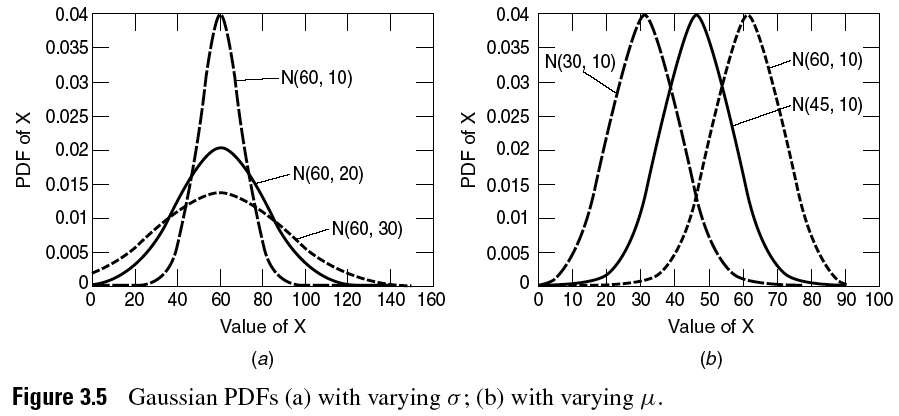
\includegraphics[width=.75\textwidth]{03_05}
\end{frame}

\begin{frame}
  \frametitle{CDF of a normal distribution}
  \pause

  \begin{itemize}[<+->]
  \item The CDF of a normal distribution is the integral of the PDF:
    \begin{equation}
      F_{X}(x) = P(X\le x) =
      \int_{-\infty}^{x} f_{x}(x)dx = \pause  \int_{-\infty}^{x}  \fr{1}{\sigma\sqrt{2\pi}}e^{-\fr{1}{2}\lt(\fr{x-\mu}{\sigma}\rt)^2} dx
    \end{equation}
    \medskip

  \item There is no closed-form solution to this integral

    \medskip
    
  \item So, in texts/tables, we denote the \textbf{\rd standard normal} CDF as $\Phi(z)$, where:
    \begin{equation}
      \Phi(z) =   \int_{-\infty}^{z} f_{Z}(z) \fr{1}{1\sqrt{2\pi}}e^{-\fr{1}{2}z^2} dz \pause = P(Z \le z)
    \end{equation}
    where \pause

    \begin{equation}
    z = \frac{x - \mu}{\sigma}
  \end{equation}

  \item The standardized normal variable $z$ is often referred to as the $Z$-score
  \end{itemize}
\end{frame}

\begin{frame}
  \frametitle{Example 1: Normal distribution parameters}
  \pause
  \begin{enumerate}[\bf (a)] \pause
  \item   A random variable $X$ is normally distributed as: $X\sim \mathcal{N}(\mu = 0,\sigma^{2}= 1)$. What are the mean and standard deviation of this distribution?
    \pause
    {\gr Mean: $\mu = 0$, standard deviation: $\sigma = 1$} \pause

  \item  A random variable $X$ is normally distributed as: $X\sim \mathcal{N}(2, 4)$. What are the mean and variance of this distribution? \pause
    {\gr  Mean: $\mu = 2$, standard deviation: $\sigma = \sqrt{4} = 2$} \pause

  \item If $X\sim\mathcal{N}(10, 4)$, what is the $Z$-score of a sample $x=5$? \pause
    {\gr
      \begin{eqnarray*}
        z &=& \fr{x - \mu}{\sigma} = \pause \fr{5 - 10}{\sqrt{4}} \\\pause
        &=& -\fr{5}{2} = \boxed{-2.5}
      \end{eqnarray*}
      \pause
      This means that the sample $x=5$ is 2.5 standard deviations below the mean
      }
  \end{enumerate}
\end{frame}
\begin{frame}
  \frametitle{Standard deviation of a normal distribution}\pause
  \begin{minipage}{.4\linewidth}
    The probabilities of a normal r.v.\ within $\pm1$, $\pm2$ and $\pm3$ standard deviations are
    68.3\%, 95.4\% and 99.7\%, respectively.    
  \end{minipage}\quad
  \begin{minipage}{.55\linewidth}
    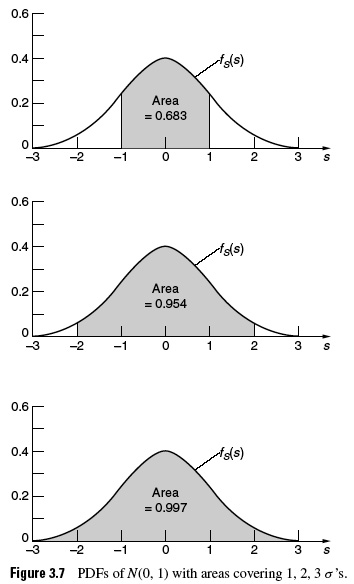
\includegraphics[width=.7\textwidth]{03_07}    
  \end{minipage}

\end{frame}

\begin{frame}
  \frametitle{Standard normal distribution}

  If a random variable $X$ has a normal distribution $\mathcal{N}(\mu,\sigma^2)$, then the r.v. $Z$ has a \alert{standard normal distribution} if

  \begin{equation}
    \label{eq:2}
    Z = \fr{X - \mu}{\sigma} \sim \mathcal{N}(0,1)
  \end{equation}

  \pause

  The standardized normal therefore has a mean of 0 and variance of 1. \pause
  Its PDF is thus:
  
  \begin{equation}
    \label{eq:3}
    f_Z(z) = \fr{1}{\sqrt{2\pi}}e^{-\fr{1}{2}z^2} \quad -\infty < z < \infty
    \end{equation}

    \pause

    The CDF $\Phi$ of the standard normal variate $Z$ is given by:
    \begin{equation}
      \label{eq:6}
      \Phi(z) = F_Z(z)
    \end{equation}
\end{frame}

\begin{frame}
  \frametitle{Probability of a normal random variable}\pause
  
  The probability that a normal r.v.\ lies within a certain interval is given by the {\it area} under the PDF in that interval. (In this figure, $S/s$ and $Z/z$ are interchangeable)
  \pause
  
  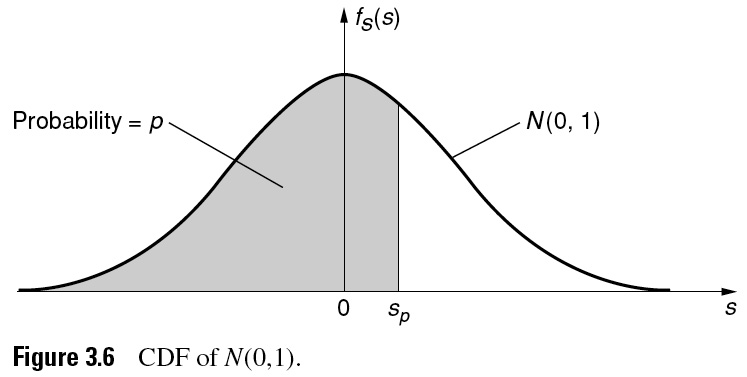
\includegraphics[width=.8\textwidth,trim=0 34 0 0, clip]{03_06}

  \pause

  \begin{itemize}[<+->]
  \item Recall that the area under the PDF within a given interval is the CDF evaluated in that range
  \item Thus, in the above figure: $p = P(Z \le z_p) = \Phi(z_p)$
  \item And, $z_p = \Phi^{-1}(p)$
  \end{itemize}
\end{frame}

\begin{frame}
  \frametitle{Probability of a normal random variable (cont.)}\pause

  Given a normal r.v.\ $X \sim \mathcal{N}(\mu,\sigma^2)$: \pause

  \begin{equation}
    \label{eq:9}
    P(a < X \le b) = \fr{1}{\sigma\sqrt{2\pi}}\int_a^b e^{-\fr12\lt(\fr{x-\mu}{\sigma}\rt)^2}dx
  \end{equation}

  \pause

  Substituting $z = \fr{x-\mu}{\sigma}$ and $dx = \sigma dz$, we obtain: \pause

  \begin{equation}
    \label{eq:10}
    P(a < X \le b) = \fr{1}{\sqrt{2\pi}}\int_{(a-\mu)/\sigma}^{(b-\mu)/\sigma} e^{-\fr12z^2}dz
  \end{equation}

  \pause

  Recognizing that the integrand is the PDF of a standard normal distribution, we have: \pause

  \begin{equation}
    \label{eq:11} \rd
    P(a < X \le b) =  \Phi\lt(\fr{b-\mu}{\sigma}\rt) -  \Phi\lt(\fr{a-\mu}{\sigma}\rt)
  \end{equation}
\end{frame}

\begin{frame}
  \frametitle{Example 2: Normal probabilities}
  \pause
  SAT scores are normally distributed as $X \sim \mathcal{N}(1100, \sigma^{2}=200^{2})$. \pause
  \begin{enumerate}[\bf(a)]
  \item What is the probability that a randomly selected student has a score that is at least 1200? \pause
    {\gr \pause
      The Z-score is $z = \fr{1200 - 1100}{200} = 0.5$ \pause

      Thus,
      \begin{eqnarray*}
      P( X \ge 1200) &=&1 -  \Phi(.5) = \pause 1 - .695 = \boxed{.3085}
      \end{eqnarray*}

    } \pause

  \item What is the probability that another randomly selected student's score is greater than 600 but less than 1200? \pause
    {\gr \begin{eqnarray*}
           P( 600 \le X < 1200) &=& \Phi\lt( \fr{1200-1100}{200}\rt)  - \Phi\lt( \fr{600-1100}{200}\rt)  \\\pause
                                &=& \Phi(.5) - \Phi(-2.5) \\\pause
                                &=& \boxed{.6853}
    \end{eqnarray*}}
  \end{enumerate}
\end{frame}

\begin{frame}
  \frametitle{Example 3: Inverse normal probabilities}
  \pause
  SAT scores are normally distributed as $X \sim \mathcal{N}(1100, \sigma^{2}=200^{2})$. \pause
  \begin{enumerate}[\bf(a)]
  \item If the probability of an SAT score lower than $x$ is 0.4, find $x$. \pause
    {\gr \pause
      \begin{eqnarray*}
        z &=& \Phi^{-1}(.4) = -.2533 = \fr{x-\mu}{\sigma} \quad \pause \text{(In MATLAB, use \texttt{norminv})} \\\pause
        \therefore x &=& z\sigma + \mu = -.2533(200) + 1100 = \boxed{1049}
      \end{eqnarray*}

    } \pause


  \end{enumerate}
\end{frame}

\begin{frame}
  \frametitle{More on the normal CDF}\pause
  
  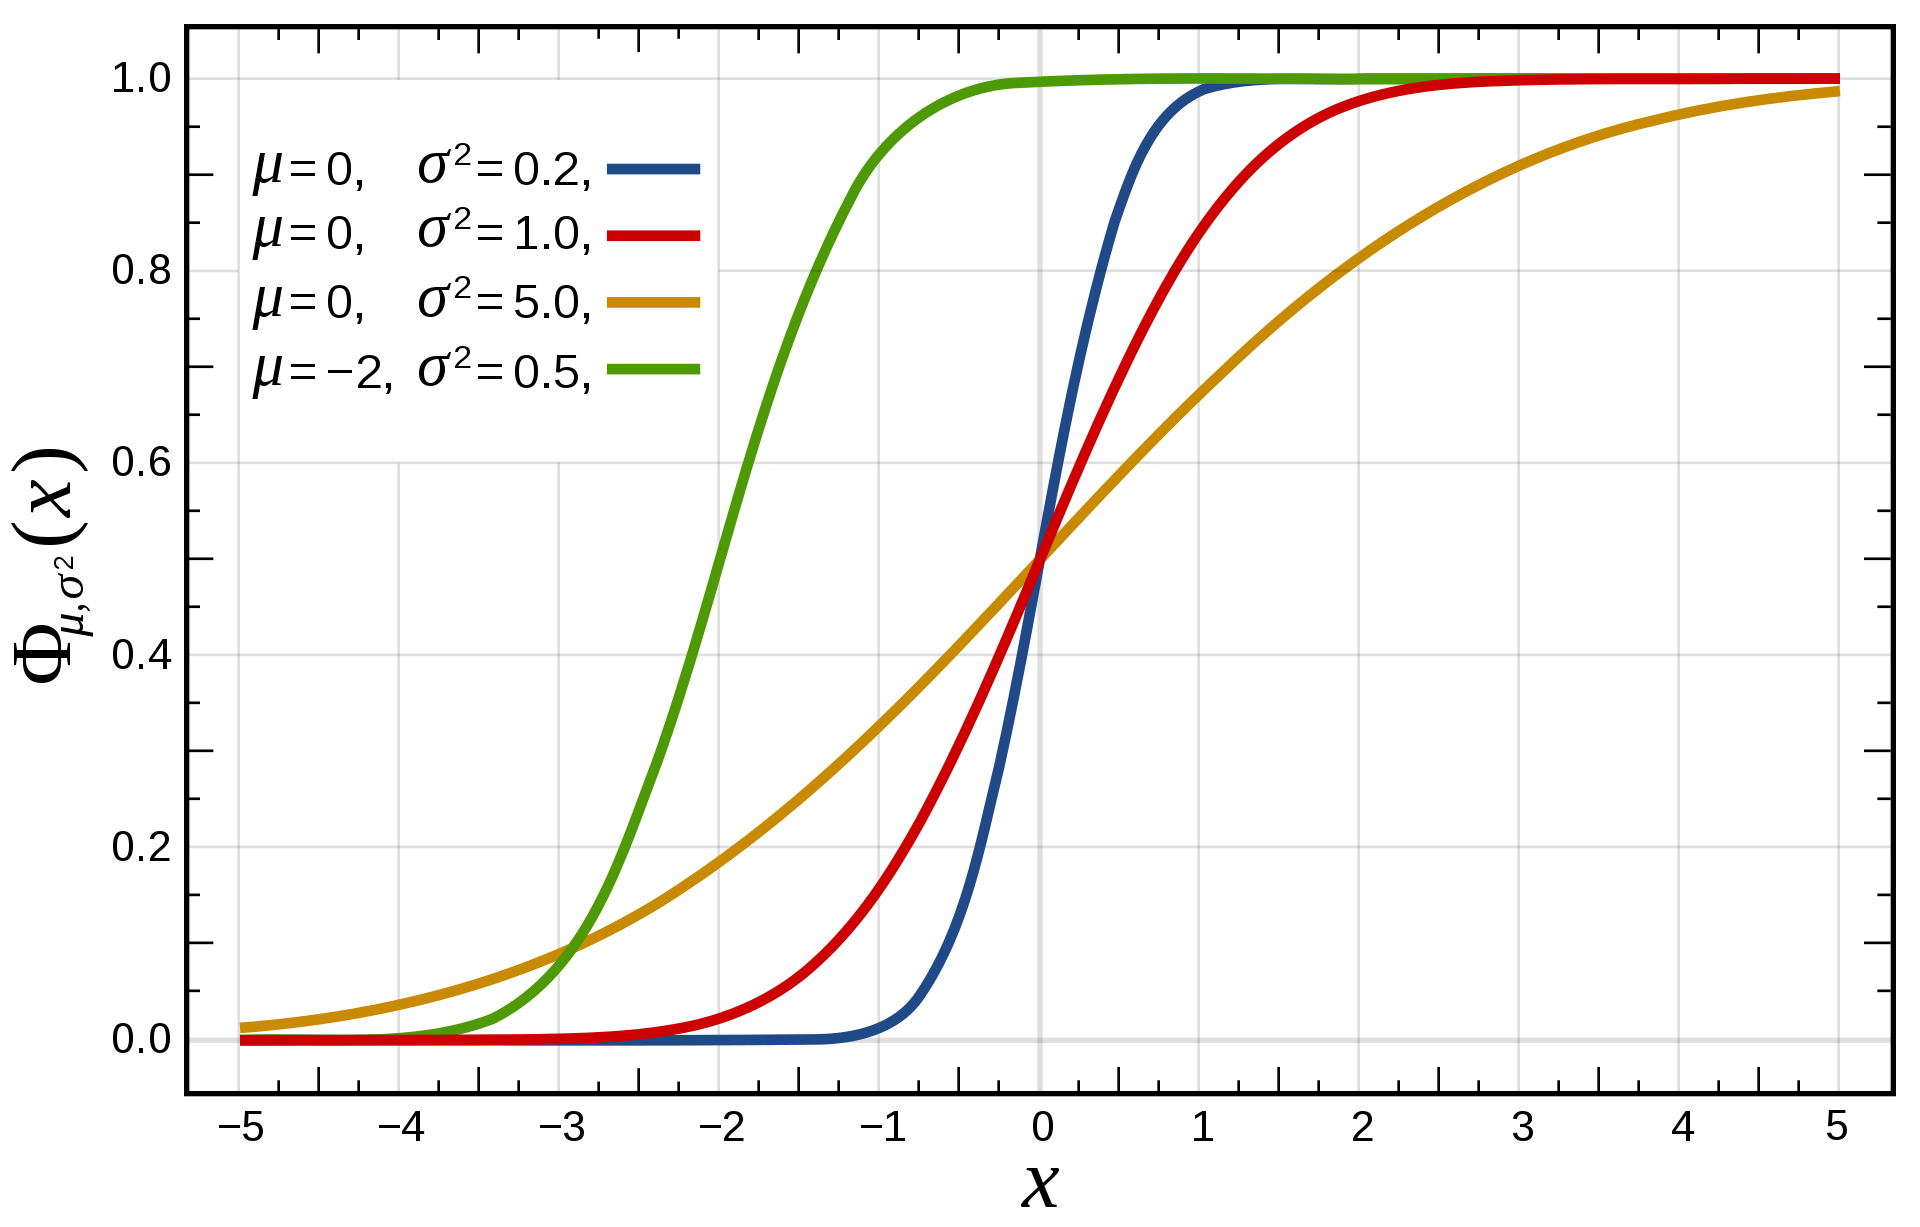
\includegraphics[width=.8\textwidth]{normdist-cdf}

  \pause

  \begin{itemize}[<+->]
  \item The standard normal CDF is the red curve in the above figure
  \item Quantiles can be read off the plot (e.g.\ the median is the value of $X$ corresponding to the $y$ value of 0.5)
  \item $\Phi(-z) = 1 - \Phi(z)$
  \item $z = \Phi^{-1}(p) = - \Phi^{-1}(1-p)$
  \end{itemize}
\end{frame}

\section{More Examples}
\begin{frame}
  \frametitle{Example 4: Probability of flooding}\pause
    The drainage from a community during a storm is a normal random variable
    estimated to have a mean of 1.2 million gallons per day (mgd) and an SD of
    0.4 mgd. If the storm drain system is designed with a maximum drainage
    capacity of 1.5 mgd:
    \begin{enumerate}[(a)]\pause
    \item What is the underlying probability of flooding during  a storm that is assumed in the design of the drainage system?
    \item Find $P(1.0 < X \le 1.6)$.
    \item Find the 90th-percentile drainage load from the community during a storm.
    \end{enumerate}
 \end{frame}


\begin{frame}
  \frametitle{Example 4: Probability of flooding (cont.)}
    \pause
    Given $\mu = 1.2$ and $\sigma = 0.4$. \pause
    \begin{enumerate}[(a)]
    \item What is the underlying probability of flooding during  a storm that is assumed in the design of the drainage system?

      \pause
      \begin{exampleblock}{Solution}
    \begin{eqnarray*}
      P(X > 1.5) &=& 1 - P(X \le 1.5) \\ \pause
                 &=& 1 - \Phi\lt(\fr{1.5 - 1.2}{0.4}\rt) \\  \pause
                 &=& 1 - \Phi(0.75) \\ \pause
                 &=& 1 - 0.7734 = 0.227
    \end{eqnarray*}
  \end{exampleblock}

    \end{enumerate}
 \end{frame}


\begin{frame}
  \frametitle{Example 4: Probability of flooding (cont.)}\pause
    \begin{enumerate}[(a)]\setcounter{enumi}{1}
    \item Find $P(1.0 < X \le 1.6)$: \pause

        \begin{exampleblock}{Solution}\pause
      \begin{eqnarray*}
          P(1.0 < X \le 1.6) &=& \Phi\lt(\fr{1.6 -1.2}{0.4} \rt) - \Phi\lt(\fr{1.0 - 1.2}{0.4}\rt) \\\pause
                           &=& \Phi(1.0) - \Phi(-0.5) \\ \pause
                           &=& 0.8413 - [1 - \Phi(0.5)] \\ \pause
                           &=& 0.8413 - (1- 0.6915) = \pause 0.533
      \end{eqnarray*}
                               \end{exampleblock}

    \end{enumerate}
 \end{frame}

\begin{frame}
  \frametitle{Example 4: Probability of flooding (cont.)} \pause
    \begin{enumerate}[(a)]\setcounter{enumi}{2}
    \item Find the 90th-percentile drainage load from the community during a storm. \pause

      \begin{exampleblock}{Solution}\pause
      \begin{eqnarray*}
        P(X\le x_{0.90}) \pause &=& \Phi\lt( \fr{x_{0.90} - 1.2}{0.40}\rt) = 0.90 \\ \pause
        \implies \fr{x_{0.90} - 1.2}{0.40}\pause  &=& \Phi^{-1}(0.90) \\ \pause
                        &=& 1.28 \\ \pause
        \therefore x_{0.90} \pause &=& 1.28(0.40) + 1.2 = \pause 1.71 \text{ mgd}
      \end{eqnarray*}
    \end{exampleblock}

    \end{enumerate}
 \end{frame}


\begin{frame}
  \frametitle{Example 5: Steel beam reliability} \pause Assume the
    variability $E$ in the lengths of steel beams is normally distributed. What
    is the precision (in terms of $\sigma$) required for a reliabiilty of
    99.7\%, given that the specified tolerance for a construction project is
    $\pm 5$ mm?\pause

    \begin{exampleblock}{Solution}\pause
    \begin{eqnarray*}
      P(-5 \le E \le 5) &=& \Phi\lt(\fr{5-0}{\sigma}\rt) - \Phi\lt(\fr{-5-0}{\sigma}\rt) = 0.997\\ \pause
      2\Phi\lt(\fr{5}{\sigma}\rt) - 1 &=& 0.997 \\ \pause
      \Phi\lt(\fr{5}{\sigma}\rt)  &=& \fr{1 + 0.997}{2} = 0.9985 \\ \pause
      \fr{5}{\sigma} &=& \Phi^{-1}(0.9985) = \pause 2.97 \\ \pause
      \implies \text{The required precision is: } \sigma &=& \pause \boxed{1.68 \text{ mm}}
    \end{eqnarray*}
  \end{exampleblock}

    
\end{frame}

\section{Outlook}


\begin{frame}
  \frametitle{Recap of normal distribution}
  \pause

  \begin{itemize}
  \item The {\gr PDF} of the normal distribution (parameters $\mu$ and $\sigma^{2}$) is given by \pause
    \begin{equation}\gr
      f_{X}(x) = \fr{1}{\sigma\sqrt{2\pi}}\exp\lt[\fr{1}{2}\lt(\fr{x - \mu}{\sigma}\rt)^{2}\rt]
    \end{equation}

  \item  The parameters of a normal distribution $\mathcal{N}(\mu,\sigma^{2})$ correspond to its mean and variance, respectively.
    \pause
    
  \item There is no closed-form solution to the integral of the normal CDF
    \pause
    
  \item Instead, it is customary to standardize a normal variable to its {\bl ``Z-score''}:\pause
    \begin{equation}\bl
      Z = \fr{X - \mu}{\sigma}
    \end{equation}
    \pause
  \item The mean and variance of the standard normal distribution are 0 and 1, respectively.
    \pause
    
  \item The symbol {\og $\Phi$ (``phi'')} is used to represent the CDF of the {\og \textit{standard} normal distribution}, whose
    values can be looked up in a table.
    \pause
    
  \item In MATLAB, the \texttt{\rd normcdf(x, mu, sigma)} and \texttt{\rd norminv(p, mu, sigma)} can be used to compute
    probabilities and inverse CDFs of the normal distribution, respectively.
  \end{itemize}
\end{frame}
%\begin{frame}[allowframebreaks]
%   \frametitle{References}
%   \AtNextBibliography{\scriptsize}
%   \setbeamertemplate{bibliography item}[text]
%   \printbibliography[heading=none]
  
% \end{frame}

%\printbibliography
\end{document}
%%% Local Variables:
%%% mode: latex
%%% TeX-master: t
%%% End:
